\chapter{Enhancement of Active Shape Model Using Color Information}
\label{colorModeling} The ASM approach represents a target structure
by a parameterized statistical model. By choosing the model
parameters, different variations of a target shape can be obtained.
In this subsection, first we review the theoretical background of
the ASM and subsequently we will present our method for improving
the technique.

In the ASM technique, the location of $n$ landmark points (e.g.
facial features in our study), are annotated on a set of training
images by a human expert. This set of points is represented by a
vector $X = (x_1,y_1, \dots, x_n,y_n)^T$, where $x_i$ and $y_i$ are
the coordinates of the $i^{th}$ landmark. Then, a model that
incorporates the variations in shape over the training set is
represented as follows: \beq X \approx \bar{X} + P~b \eeq The vector
$\bar{X}$ contains the mean values of the coordinates of the
annotated data, $P$ is a matrix of the first $t$ eigenvectors of the
covariance matrix of the annotated data, and $b$ is a vector that
defines the model parameters. The variance of the $i^{th}$
parameter, $P_i$, across the training set is given by the
corresponding eigenvalue $\lambda_i$. By limiting the parameter
$b_i$ in the range of $\pm3\sqrt{\lambda_i}$, we ensure that the
generated shape is similar to those in the original training set. To
apply the created shape model to a given target shape, we need to
find a transformation to move from the model coordinate system to
the image coordinate system. Typically, this is achieved by a
similarity transformation defining the translation $(X_t, Y_t)$,
rotation $\theta$, and scale $s$. Therefore, the position of the
model points , $X$, in the image are given by: \beq X =
T_{X_t,Y_t,\theta,s}(\bar{X} + P~b) \eeq

For a given new image, the ASM is performed to find where the target
object lies on the image. Therefore, we need to find the optimum
parameters of the ASM that best fit of the model to the target
structure. Generally, this optimization problem is solved
iteratively \cite{Cootes_1}. At the first step, the model is
initialized by the mean shape. Afterwards, a region of the image
around each feature point is examined to find the best nearby match
(e.g., searching along the profile line for the edge locations). In
the next step, the parameters $X_t, Y_t, s, \theta$, and $b$ are
updated to best fit the new found points. Then, the constraint
$|b_i| < 3\sqrt{\lambda_i}$ is applied to the parameters $b_i$.
These steps are repeated until there is no significant change in the
shape parameters.

\section{Shape Model Initialization and Face Alignment Using 2-D
Affine Transformation } As we mentioned in subsection
\ref{asm_and_limmitation}, the initialization of the ASM is very
important. With poor initialization, the search process may either
fail or become slow. Therefore, a good initialization would help in
finding the optimum solution in less iterations. We use our
algorithm in \cite{Mottaleb02} to find the centers of the mouth and
the two eyes. Figure \ref{fig_initialization} shows the extracted
locations of the eyes and the mouth in a given color face image
using this method. We use these three points to obtain the affine
parameters in Equation \ref{affine_eq} to initialize the shape model
for the image.

For a 3-D object like the face, since it may have some pose
variations in the captured images, a similarity transformation with
4 degrees of freedom is not effective especially when there are
large pose variations. When the head is rotated to the left or
right, this problem is more severe. To solve this problem, we use a
2-D affine transformation with 6 degrees of freedom, given by
Equation \ref{affine_eq}, to align the extracted feature points in
the image coordinate system with the points represented by the model
coordinate system. \beq \label{affine_eq} \left(\begin{array}{ccc}
x^\prime\\y^\prime\\1\end{array}\right)=\left[\begin{array}{lcr}
a_{11} &~ a_{12}&~ t_x\\ a_{21} &~ a_{22} &~ t_y\\
0 &~ 0 &~ 1\end{array}\right] \left(\begin{array}{ccc}
x\\y\\1\end{array}\right)\eeq To find the parameters of the 2-D
affine transformation, we need at least three corresponding points,
which are not conlinear.

\begin{figure}[tbp]
\begin{center}
\includegraphics[scale=0.8]{./chapters/figures/initial.eps}
\caption{Detecting the center of the mouth and the eyes as the
salient features for initialization.} \label{fig_initialization}
\end{center}
\end{figure}
%%%%%%%%%%%%%
\section{Improvement of The Local Structure Model} In the
original ASM, the local structure of a feature point is modeled by
assuming that the normalized first derivative of the pixel intensity
values along a profile line satisfies a multivariate Gaussian
distribution. This gives a statistical model for the profile around
the point. As shown in Figure \ref{fig_profile}, a sampled profile,
$g_s$, is matched to a reference model by searching along the
profile line that goes through the point and finding the best fit.
This is achieved by calculating the Mahalanobis distance: \beq
\label{Mahalanobis_eq}f(g_s) = (g_s - \bar{g})^T\Sigma^{-1}(g_s -
\bar{g}) \eeq where $\bar{g}$ is the mean value and $\Sigma$ is the
covariance matrix.

In this dissertation, we assumed that the normalized first
derivative of three channel values (i.e., Hue, Saturation, and
Value) along a profile line for each individual channel satisfies a
multivariate Gaussian distribution. Then, we use a weighted sum of
Mahalanobis distances for the three color channels to find the best
match for the feature points. Similar to Equation
\ref{Mahalanobis_eq}, the best matching of a probe sample,
$g_{hsv}$, in HSV color space to a reference model is carried out
by: \beq f(g_{hsv}) = \sum_{i \in \{h,s,v\}} w_i.(g_i -
\overline{g_i})^T\Sigma^{-1}_i(g_i - \overline{g_i}) \eeq where
$w_i$ is the weighting factor for the $i^{th}$ component of the
Gaussian model with unit sum.
%%%%%%%%%%%%%
\begin{figure}[tbp]
\begin{center}
\includegraphics[scale=0.8]{./chapters/figures/profile.eps}
\caption{Searching along a sampled profile to find the best fit.}
\label{fig_profile}
\end{center}
\end{figure}
%%%%%%%%%%%%%
\section{Enhancement of the Location of Features Around the Lips}
\label{Section_lips} To accurately localize the feature points
around the lips, we segment the lips region from the facial skin
region. This is achieved by classifying each pixel, I(h,s,v), in HSV
color space, either as facial skin or lips. This classification
starts by applying the Fisher Discriminant Analysis (FDA) technique.
FDA is a data analysis technique that provides more class
separability than Principal Component Analysis (PCA), which provides
better data representation. By applying FDA to each pixel of the
color image, I(h,s,v), we obtain a scalar function that can be used
to discriminate between the two classes: facial skin and lips. This
function is calculated by using the within-class scatter matrix and
is defined as: \beq\label{FDA_equation} Fisher(I) = W . I^T \eeq
where $I$ is a given pixel value. The projection vector $W$, is
calculated by: \beq W = S_W^{-1}(m_1 - m_2) \eeq The within class
scatter matrix $S_W$, is: \beq S_W = S_1 + S_2 \eeq and \beq S_i =
\sum(I - m_i)(I - m_i)^T \eeq The sample mean vector of each class,
$m_i$, is defined as: \beq m_i = \frac{1}{n_i} \sum_{I \epsilon
D_i}I\eeq Where $D_i$ is the set of the pixels in $i^{th}$ class and
$n_i$ is the number of the pixels in the class.

To learn the projection matrix $W$, we obtain a color database of
facial images and manually extract patches of lips and facial skin
regions. Then, the matrices $S_i$ and $m_i$ are calculated for the
two classes of facial skin and lips. For a given test image, we
apply the FDA function (Eq. \ref{FDA_equation}) and apply threshold
to the result to segment the lips from the facial skin. Figure
\ref{fig:lip_detection} shows the results of the different steps for
lips detection applied to a sample image in our database using FDA.
Figure \ref{fig_lip_a} is the original image, Figure \ref{fig_lip_b}
shows the result of applying FDA, Figure \ref{fig_lip_c} shows the
result of thresholding. The value of the threshold is obtained by a
small training set different from the images used in the experiment
Section. The result of applying morphological operators to remove
noise and fill holes is shown in \ref{fig_lip_d}.
\begin{figure}[tbp]
  \begin{center}
    \mbox{
      \subfigure[]{\includegraphics [scale = 1]{./chapters/figures/lip_1.eps}\label{fig_lip_a}}
      \subfigure[]{\includegraphics [scale = 1]{./chapters/figures/lip_4.eps}\label{fig_lip_b}}
      }
      \mbox{
      \subfigure[]{\includegraphics [scale = 1]{./chapters/figures/lip_3.eps}\label{fig_lip_c}}
      \subfigure[]{\includegraphics [scale = 1]{./chapters/figures/lip_4.eps}\label{fig_lip_d}}
      }
\caption{Lips detection using FDA. (a) Original image.(b) Result of
FDA classification. (c) Result of thresholding. (d) Result of
applying morphological operators.}\label{fig:lip_detection}
\end{center}
\end{figure}
%%%%%%%%%%%%%
The following summaries our iterative approach for facial features
extraction using the enhanced active shape model:
\begin{table}
\begin{enumerate}
\item Extract the centers of the eyes and the mouth \cite{Mottaleb02}.
\item Initialize the shape model based on the extracted three points from step
1.
\item Calculate the shape parameters, $b$.
\item Examine a region of the image around each point, $(x_i, y_i)$, to
find the best nearby match for that point using the color model.
\item Use lips detection to tune the feature points around the
mouth.
\item Update the parameters of the affine transformation
($a_{11}, a_{12}, a_{21}, a_{22}, t_x, t_y$) to best fit the new
found locations of the instance, $X$, of the target model.
\item Apply the constraints to the parameters, $b$, to ensure reasonable
shapes (i.e. $|b_i| \le 3\sqrt{\lambda_i}$).
\item Go to step 3 and repeat until convergence.
\end{enumerate}
\end{table}
%%%%%%%%%%%%%
